\chapter{Let's get more confident with our little friend op-amp}
We designed an inverting amplifier with a gain variable by the use of a trimmer. The second circuit designed was a non-inverting summing amplifier with unitary gain. We then built a current source generator of $1$ mA and tested it with various loads. Next we tested the efficacy of the emitter follower configuration in mismatching the source's impedence. At last we designed a differential amplifier with a predetermined gain.

\section{Materials}
\begin{itemize}
\item Operational amplifier uA741
\item Resistors and trimmers
\item Power supply RIGOL DP831A
\item Waveform generator RIGOL DG1032
\item Multimeter RIGOL DM3068
\item Oscilloscope RIGOL MS02102A
\item Two capacitors of nominal value of $100$nF
\end{itemize}

\section{Experiment setup}
In each circuit we powered the op-amp with a $\pm15$ V DC voltage and, in order to reduce possible noises, we added two 100nF capacitors connecting the op-amp's pins for the power supply with the ground. The input signal had a frequency of 100 Hz and a peak-peak voltage of 1V except for the differential amplifier. For every specific circuit we designed them as follow:
\begin{itemize}
\item Inverting amplifier: we placed a 10k$\Omega$ trimmer along the feedback branch in series to a resistor $R_f = 983.9 \pm 0.1 \Omega$. In order to have a minimum gain of 5, we used $R_{in} = 199.84\pm 0.03 \Omega$ as in figure \eqref{Non-inverting variable amplifier}.
\item Summing amplifier: caring for the simplest calculations, we used $R_1 = 1484.7 \pm 0.2 \Omega \simeq R_2= 1483.5\pm 0.2\Omega$ so the equation comes to be $\displaystyle v_o = \frac{v_1+v_2}{2}\left(1+\frac{R_4}{R_3}\right)$. In order to obtain as output the inputs sum, we had to choose $R_3 = R_4 = 1001.3 \pm 0.1 \Omega$. The inputs $v_1$ and $v_2$ are the same 100 Hz, 1 V peak-peak sine wave signal.
\begin{figure}[H]
\centering
\begin{minipage}{.5\textwidth}
\centering
\begin{circuitikz}
\draw(0,0) node[op amp] (opamp) {}
	%(opamp.+) node[left] {$v_+$}
	(opamp.+) ++ (-.3,0) node[ground] {} -- (opamp.+) 
	(opamp.out) to[short] (1.8,0) node[right] {$v_o$}
	(opamp.down) ++(0,-.7) node[below] {$-v_{cc}$} -- (opamp.down)
	(opamp.up) ++ (0,.7) node[above] {$+v_{cc}$} -- (opamp.up)
	(opamp.down) ++ (0,-.25)to[C,/tikz/circuitikz/bipoles/length=1cm] (1,-.8)node[ground,rotate = 90,yshift = 1em] {}
	(opamp.up) ++ (0,.25)to[C,/tikz/circuitikz/bipoles/length=1cm] (1,.8)node[ground,rotate = 90,yshift = 1em] {};
	\draw(-4,-1) to[sV,l=$v_{in}$] (-4,.5) to[R=$R_{in}$] (-2,.5) to[short] (opamp.-);
	\draw(-4,-1) node[ground] {};
	\draw(-1.5,.5) to[short](-1.5,2.2) to[R=$R_f$](0,2.2) to[vR=$R_x$] (1.5,2.2)  to[short](1.5,0);
\end{circuitikz}
\caption{Inverting variable amplifier}\label{Non-inverting variable amplifier}
\end{minipage}%
\begin{minipage}{.5\textwidth}
\centering
\begin{circuitikz}
\draw(0,0) node[op amp] (opamp) {}
	%(opamp.+) node[left] {$v_+$}
	%(opamp.+) ++ (-.3,0) node[ground] {} -- (opamp.+) 
	(opamp.out) to[short] (1.8,0) node[right] {$v_o$}
	(opamp.down) ++(0,-.7) node[below] {$-v_{cc}$} -- (opamp.down)
	(opamp.up) ++ (0,.7) node[above] {$+v_{cc}$} -- (opamp.up)
	(opamp.down) ++ (0,-.25)to[C,/tikz/circuitikz/bipoles/length=1cm] (1,-.8)node[ground,rotate = 90,yshift = 1em] {}
	(opamp.up) ++ (0,.25)to[C,/tikz/circuitikz/bipoles/length=1cm] (1,.8)node[ground,rotate = 90,yshift = 1em] {};
	\draw(-4,-.5)node[left]{$v_1$} to[R=$R_{1}$,o-] (-2,-.5) to[short] (opamp.+);
	\draw(-4,-1.5)node[left]{$v_2$} to[R=$R_{2}$,o-] (-2,-1.5) to[short] (-2,-.5);
	\draw(opamp.-) -- (-1.5,.5) to[short](-1.5,2.2) to[R=$R_4$](1.5,2.2) to[short](1.5,0);
	\draw(-1.5,2.2) to[R=$R_3$] (-4,2.2)node[ground] {};
\end{circuitikz}
\caption{Non-inverting summing amplifier, unitary gain}
\end{minipage}
\end{figure}
\item Emitter follower test: at first we built a circuit without the emitter follower using an input impedence of $R=100.2\pm 1\, \text{k}\Omega$ and a load of $R_L=19.8\pm 0.2\text{k}\Omega$.  Then we added the op-amp stage and compared the output measurements in the 2 different cases.
\begin{figure}[H]
\centering
\begin{minipage}{.5\textwidth}
\centering
\begin{circuitikz}
\draw(0,0)node[ground]{} to[sV] (0,2) to[R=$R$,-o]node[right,xshift=.8em] {$v_o$} (2,2);
\draw(1.8,2) to[R=$R_L$](1.8,0)node[ground]{};
\end{circuitikz}
\caption{Test circuit without follower}
\end{minipage}%
\begin{minipage}{.5\textwidth}
\centering
\begin{circuitikz}
\draw(0,0) node[op amp] (opamp) {}
	%(opamp.+) node[left] {$v_+$}
	(opamp.+) ++ (-.3,0) node[ground] {} -- (opamp.+) 
	(opamp.out) to[short,-o] (1.8,0) node[right] {$v_o$}
	(opamp.down) ++(0,-.7) node[below] {$-v_{cc}$} -- (opamp.down)
	(opamp.up) ++ (0,.7) node[above] {$+v_{cc}$} -- (opamp.up)
	(opamp.down) ++ (0,-.25)to[C,/tikz/circuitikz/bipoles/length=1cm] (1,-.8)node[ground,rotate = 90,yshift = 1em] {}
	(opamp.up) ++ (0,.25)to[C,/tikz/circuitikz/bipoles/length=1cm] (1,.8)node[ground,rotate = 90,yshift = 1em] {};
	\draw(-4,-1) to[sV,l=$v_{in}$] (-4,.5) to[R=$R$] (-2,.5) to[short] (opamp.-);
	\draw(-4,-1) node[ground] {};
	\draw(-1.5,.5) to[short](-1.5,2.2)to[short] (1.5,2.2)  to[short](1.5,0);
	\draw(1.6,0) to[R=$R_L$] (1.6,-2)node[ground]{};
\end{circuitikz}
\caption{Test circuit with follower}
\end{minipage}
\end{figure}
\item Current generator: the aim of this circuit is to generate a stable fixed current indipendent from the load. We generated a $1$mA current using a DC voltage source of 5V and a 4.9693 $\pm$ 0.7k$\Omega$ resistor. The load was simulated with a trimmer. 
\item Differential amplifier: the full equation of the circuit in figure \eqref{differential amplifier} is the following:
\[v_o = \frac{R_F}{R_1}\left[\frac{v_b}{1+R_f/Ry}\left(1+\frac{R_1}{R_F}\right)-v_a\right]\]
first we set to ground $v_b$, in this way we were able to set up the gain of the circuit (we chose it to be $A=\frac{R_F}{R_1}=2$ with $R_F =3\pm 0.2\, \text{k}\Omega$ (5\% error of nominalvalue)). After that we put the same signal of $v_a$ in $v_b$ with a resistor $R_f$ and a variable resistor $R_y$ made with $R_2$ in series with a trimmer. We tweaked the trimmer in order to get the output as close to zero as possibile (Figure \eqref{Tuning_diff-amplifier}). This means having in the equation $R_f/R_y = R_1/R_F$ so that the new output would exaclty be what we want, i.e. $v_0 = A(v_b-v_a)$. For the amplifier test we used $v_a= 5$V DC and for $v_b$ a sine wave 1V peak-peak 100Hz with an offset of 5V.
\end{itemize}
\begin{figure}[H]
\centering
\begin{minipage}{.5\textwidth}
\centering
\begin{circuitikz}
\draw(0,0) node[op amp] (opamp) {}
	%(opamp.+) node[left] {$v_+$}
	(opamp.+) ++ (-.3,0) node[ground] {} -- (opamp.+) 
	(opamp.out) to[short] (1.8,0) node[right] {$v_o$}
	(opamp.down) ++(0,-.7) node[below] {$-v_{cc}$} -- (opamp.down)
	(opamp.up) ++ (0,.7) node[above] {$+v_{cc}$} -- (opamp.up)
	(opamp.down) ++ (0,-.25)to[C,/tikz/circuitikz/bipoles/length=1cm] (1,-.8)node[ground,rotate = 90,yshift = 1em] {}
	(opamp.up) ++ (0,.25)to[C,/tikz/circuitikz/bipoles/length=1cm] (1,.8)node[ground,rotate = 90,yshift = 1em] {};
	\draw(-4,-.8) to[battery1] (-4,.5) to[R=$R_{3}$] (-2,.5) to[short] (opamp.-);
	\draw(-4,-.5) node[ground] {};
	\draw(-1.5,.5) to[short](-1.5,2.2) to[vR=$R_x$] (1.7,2.2)to[myvoltmeter](1.7,0);
\end{circuitikz}
\caption{Current source generator}
\end{minipage}%
\begin{minipage}{.5\textwidth}
\centering
\begin{circuitikz}
\draw(0,0) node[op amp] (opamp) {}
	%(opamp.+) node[left] {$v_+$}
	%(opamp.+) ++ (-.3,0) node[ground] {} -- (opamp.+) 
	(opamp.out) to[short] (1.8,0) node[right] {$v_o$}
	(opamp.down) ++(0,-.7) node[below] {$-v_{cc}$} -- (opamp.down)
	(opamp.up) ++ (0,.7) node[above] {$+v_{cc}$} -- (opamp.up)
	(opamp.down) ++ (0,-.25)to[C,/tikz/circuitikz/bipoles/length=1cm] (1,-.8)node[ground,rotate = 90,yshift = 1em] {}
	(opamp.up) ++ (0,.25)to[C,/tikz/circuitikz/bipoles/length=1cm] (1,.8)node[ground,rotate = 90,yshift = 1em] {};
	\draw(-4,-.5)node[left]{$v_B$} to[R=$R_{f}$,o-] (-2,-.5) to[short] (opamp.+);
	\draw((-2,-.5) to[vR=$R_{y}$] (-2,-2.5) node[ground]{};
	\draw(opamp.-) -- (-1.5,.5) to[short](-1.5,2.2) to[R=$R_F$](1.5,2.2) to[short](1.5,0);
	\draw(-1.5,2.2) to[R=$R_1$,-o] (-4,2.2)node[left] {$v_A$};
\end{circuitikz}
\caption{differential amplifier}\label{differential amplifier}
\end{minipage}
\end{figure}
\begin{figure}[H]
\centering
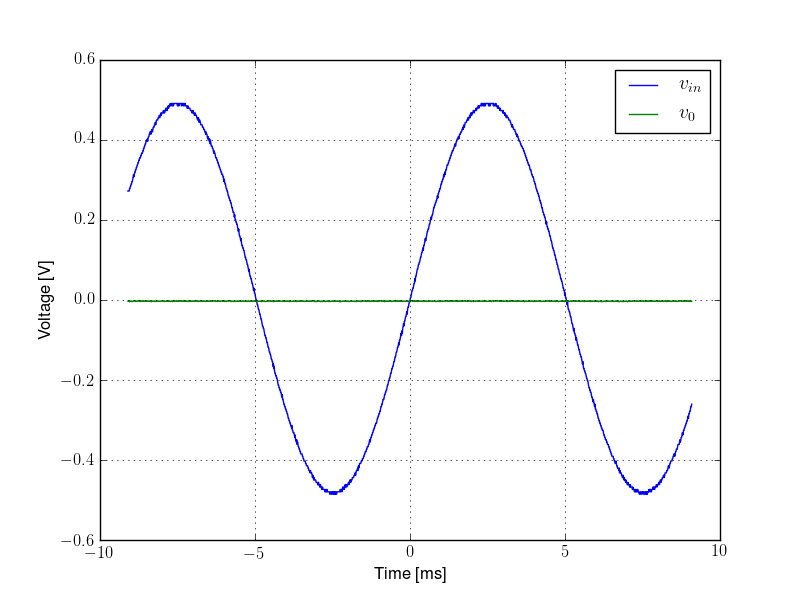
\includegraphics[width=.7\textwidth]{2/Tuning_diff-amplifier.png}
\caption{Calibration of the differential amplifier}\label{Tuning_diff-amplifier}
\end{figure}

\section{Data analysis}
\begin{figure}[H]
\centering
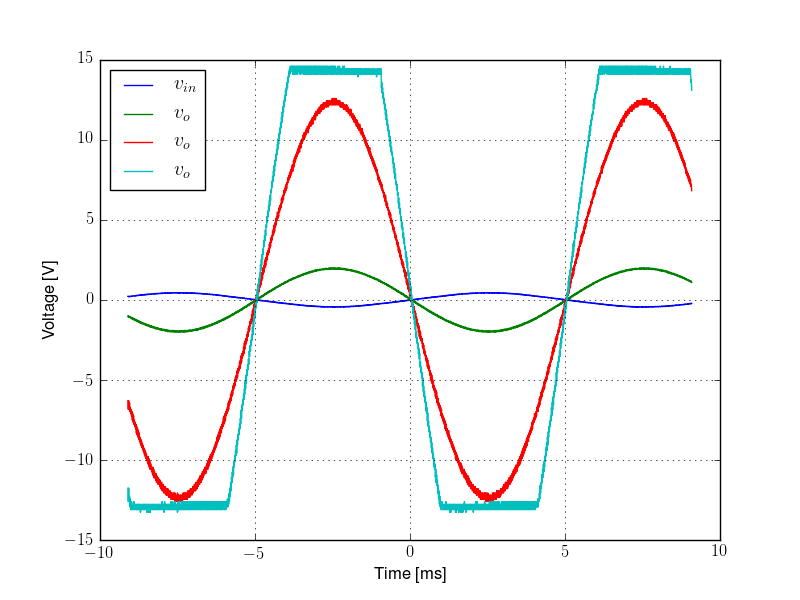
\includegraphics[width=.7\textwidth]{2/Variable_amplifier.png}
\caption{Variable amplifier}\label{Variableamplifier}
\end{figure}
In the inverting amplifier we used a trimmer in order to vary the gain, in fact the equation is:
\[v_{o} = -v_{in}\frac{R_f+R_x}{R_{in}}\]
then increasing $R_x$ cause the output to increase linearly. The output voltage is bounded by the op-amps's power supply voltage, it cannot increase further and the signal goes flat, as we can see in figure \eqref{Variableamplifier} (light blue line), this behavior is called ``Clipping''. The graphic also shows a discrepance between the absolut value of maximum and minimum voltage during the clipping: this is due to the asimmetry between \emph{pnp} and \emph{npn} transistors in the op-amp's final stage.
\begin{figure}[H]
\centering
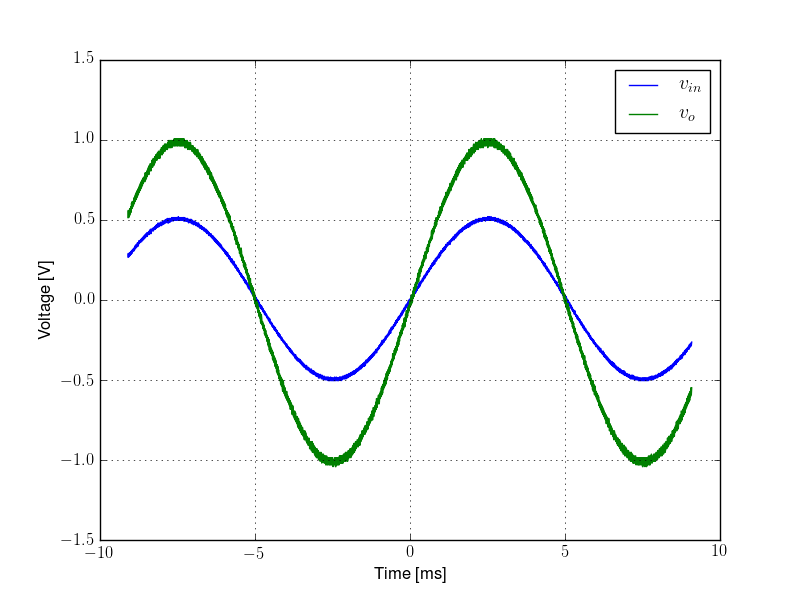
\includegraphics[width=.7\textwidth]{2/Weighted_amplifier.png}
\caption{Weighted summing amplifier}\label{Weighted_amplifier}
\end{figure}
In the non-inverting summing amplifier circuit we wanted the output to be the simple sum of the signals in entrance, that were identical: it means that the output signal must have double amplitude compared to the input one. The peak-peak voltage's theoretical expectation is $2.0496 \pm 0.0009$V while the measured one is $2.032 \pm 0.001 $V. The incompatibility is most likely due to the op-amp's non-ideality.
\begin{figure}[H]
\centering
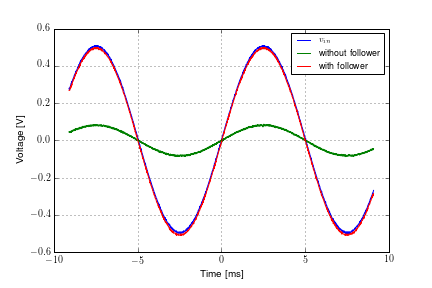
\includegraphics[width=.7\textwidth]{2/Emitter_follower_compared.png}
\caption{Emitter follower comparison}\label{Emitter_follower_compared}
\end{figure}
Let's now analyse the differences between a circuit with and without follower stage. We can see in figure \eqref{Emitter_follower_compared} that using the follower we obtain a replicated signal while without it the signal is much more shrinked due to the input impedence. We can then say that the op-amp has separated the circuit in two different parts, overshadowing to the second any impedence present in the first: this is exactly what we mean by "impedence mismatching".\\
The difference between the blue and the red line is caused once again by the non-ideality of the op-amp, probably by a non zero offset.\\
\newline
In the current generator circuit we firstly measured the output current $I_m = 1.0045 \pm 0.0006 $mA that was compatible with the expected one $I_e = \frac{v_{in}}{R_3} = 1.0062 \pm 0.0020 $mA, then we observed the indipendency from the trimmer resistence of the current value: varying the resistance the current value was always the same (at least within its uncertainty).
\begin{figure}[H]
\centering
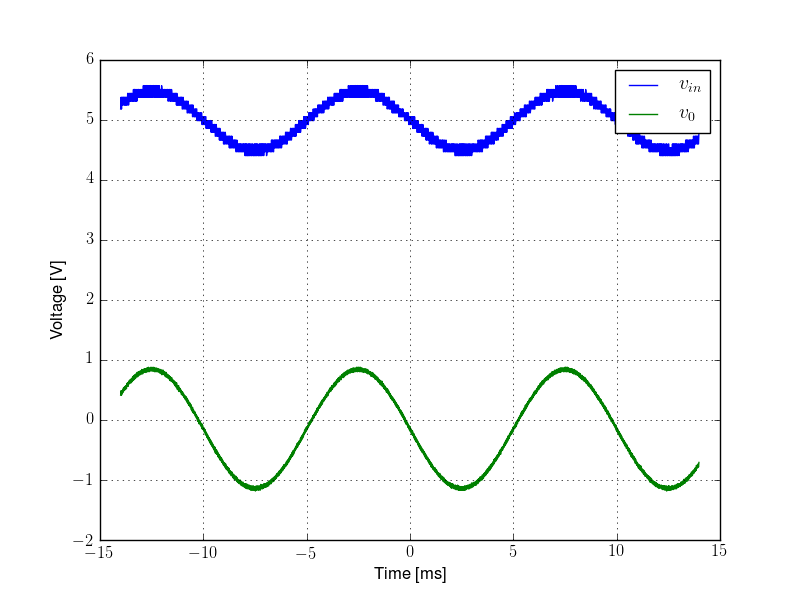
\includegraphics[width=.7\textwidth]{2/Differential_amplifier.png}
\caption{Differential amplifier}\label{Differential amplifier}
\end{figure}
In the differential amplifier circuit we measured an output cleared from the 5V DC part present in both inputs: the output consisted only in the AC component of the input, but doubled (as we can see in figure \eqref{Differential amplifier}). This is exactly how we expected the circuit to behave.
